\section{Model Evaluation}
\label{sec-evaluation}
% \begin{figure*}[!t]
%     \centering
%     \subfigure[Traditional Lens]{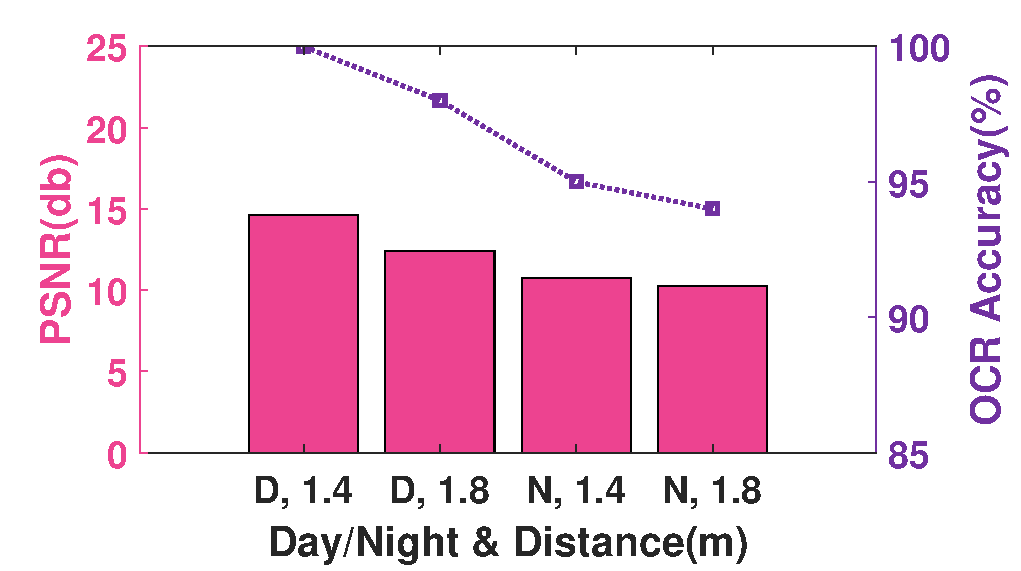
\includegraphics[width=0.24\textwidth]{./pic/data_1.pdf}\label{fig-control-1}}
%     \subfigure[Optical Lens]{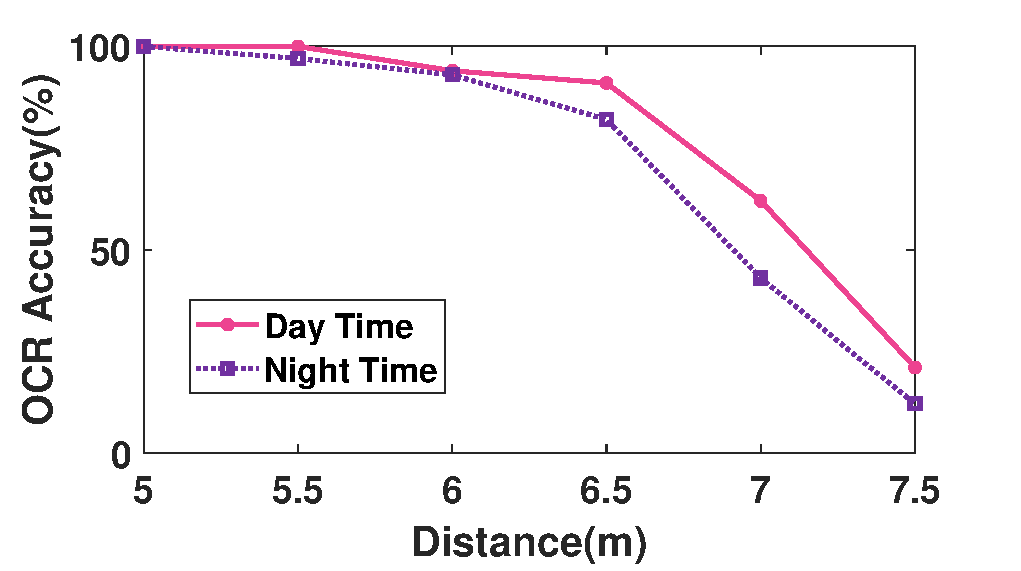
\includegraphics[width=0.24\textwidth]{./pic/data_1_2.pdf}\label{fig-control-2}}
%     \subfigure[Traditional Lens]{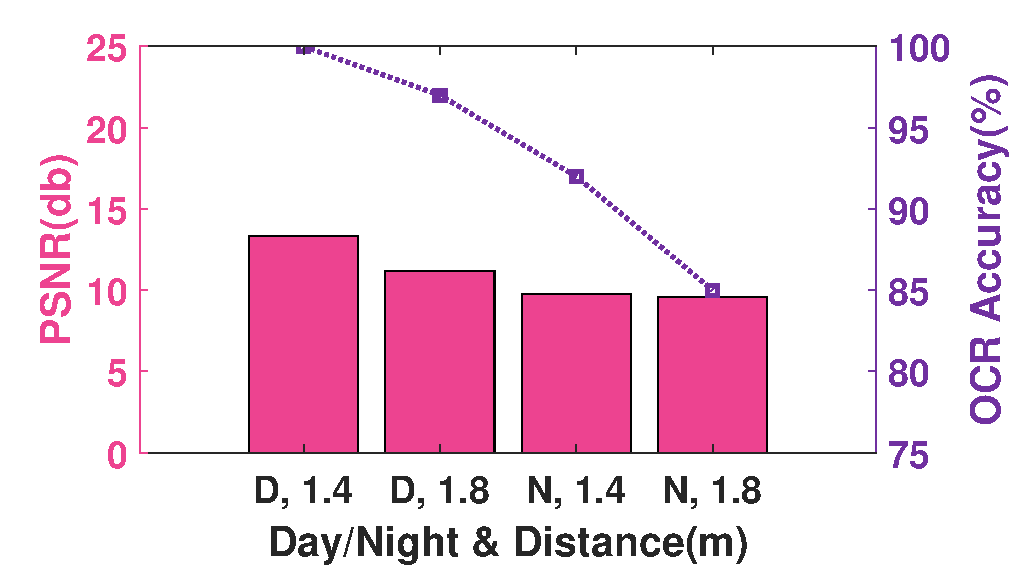
\includegraphics[width=0.24\textwidth]{./pic/data_2.pdf}\label{fig-random-1}}
%     \subfigure[Optical Lens]{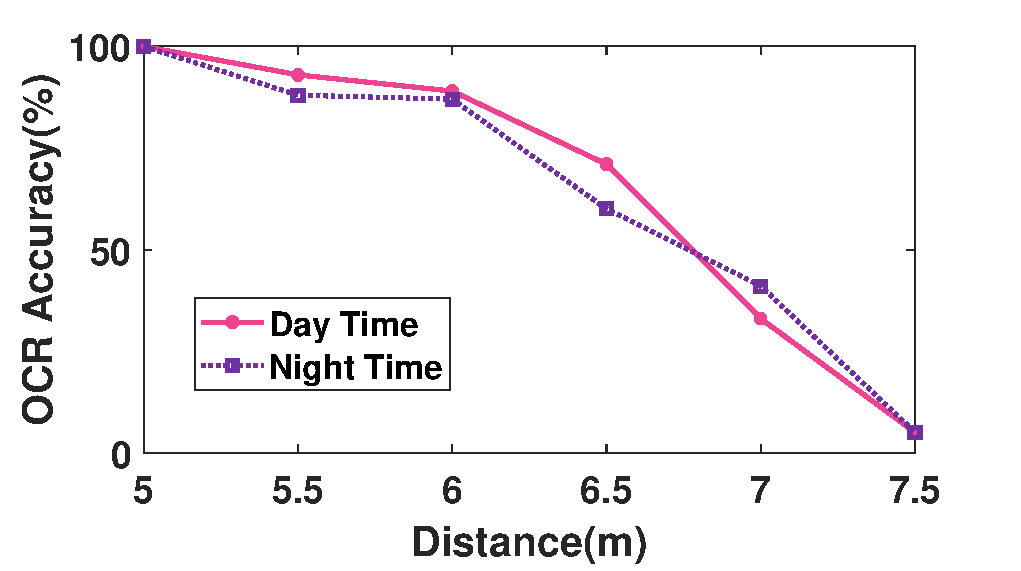
\includegraphics[width=0.24\textwidth]{./pic/data_2_2.pdf}\label{fig-random-2}}
%     \hfill
%     \caption{Performance in Controlled Environment (a,b) and Random Environment (c,d).}
%     \label{fig-performance-1}
% \end{figure*}
We evaluate the performance of the network model in different training and testing conditions. We perform the following experiments with two commercial off-the-shelf(COTS) smartphones: a Redmi 6A smartphone, with a single rear camera with 13 million pixels and digital zoom only, and a HUAWEI P40 Pro, with multiple rear cameras. The telephoto camera possess up to 5x optical zooming ability which we will utilize fully in our experiments.
 
\subsection{Performance In Controlled Environments}
% \begin{figure}[!t]
%     \centering
%     \subfigure[Traditional Lens]{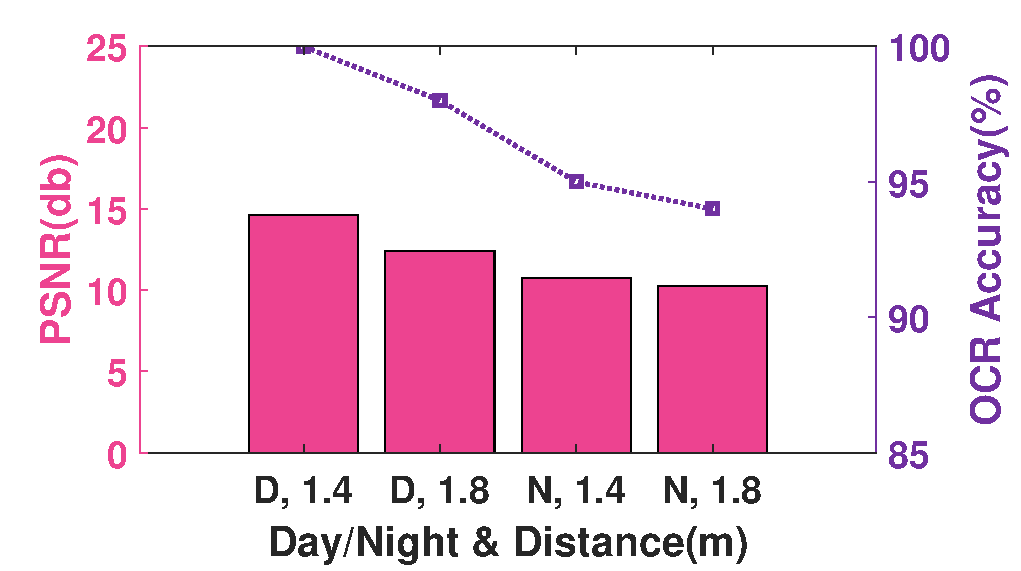
\includegraphics[width=0.40\textwidth]{./pic/data_1.pdf}\label{fig-control-1}}
%     \subfigure[Optical Lens]{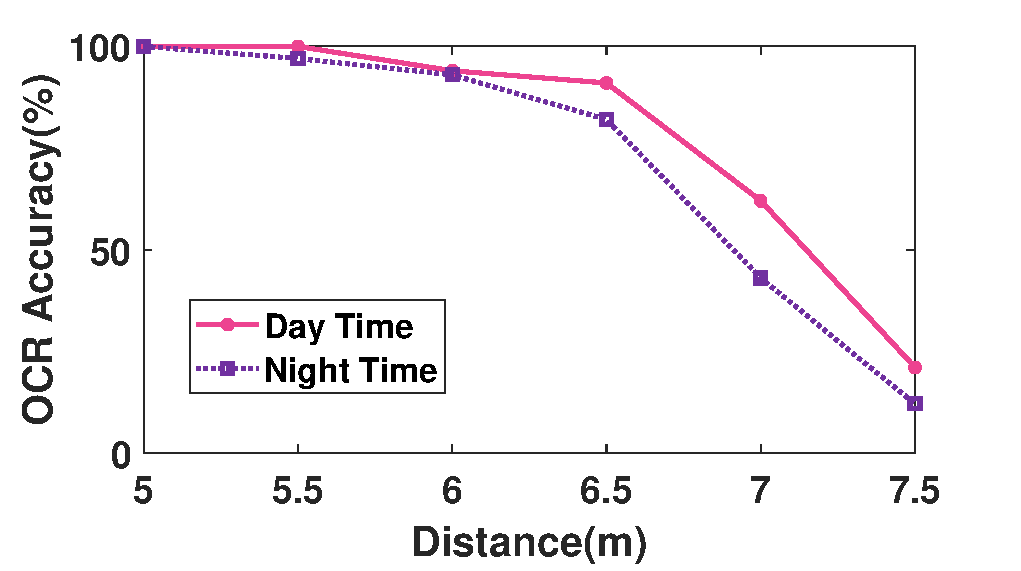
\includegraphics[width=0.40\textwidth]{./pic/data_1_2.pdf}\label{fig-control-2}}
%     \hfill
%     \caption{Performance in the controlled environment using traditional lens and optical lens.}
%     \label{fig:control}
% \end{figure}

In these experiments, we train and test the model with the images captured with exactly the same environment parameters, and used Peak Signal to Noise Ratio(PSNR) to evaluate the accuracy of the recovered images. The results are shown in Figure~\ref{fig-control-1} and Figure~\ref{fig-control-2}. Optical Character Recognition (OCR) services are also utilized to evaluate the accuracy. The traditional lens group is trained and tested at 1-2 meters distance, while the optical lens, 5-7.5 meters, where less than 5\% of the characters can be read with the naked eye. The PSNR and OCR results are shown in Fig. ~\ref{fig-control-1}.

This model can achieve an OCR accuracy above 90\% at 1.8m with traditional lens and at 6m with optical lens. Performances are relatively consistent in both day and night time, while increased distances mean less data, causing more artifacts(missing or misplaced strokes, etc.). It is the nature of Chinese characters that one mistaken stroke will largely affect its readability, leading to the result that while the pixel-wise error rises steadily with the increased distance, the accuracy will experience a drastic drop.

\subsection{Performance In Random Environments}
We train the model with data captured in different environments, as mentioned before, and test its ability in other environments. The results are shown in Figure~\ref{fig-random-1} and Figure~\ref{fig-random-2}. We can observe that the model performs best in daytime and at closer distances. For Figure~\ref{fig-random-1}, the model can still achieve an OCR accuracy above 85\% at 1.8m with traditional lens. From Figure~\ref{fig-random-2}, the OCR accuracy keeps higher than 90\% at 6m with optical lens. This verifies the efficiency of our model for environment adaption.

% \begin{figure}[!t]
%     \centering
%     \subfigure[Traditional Lens]{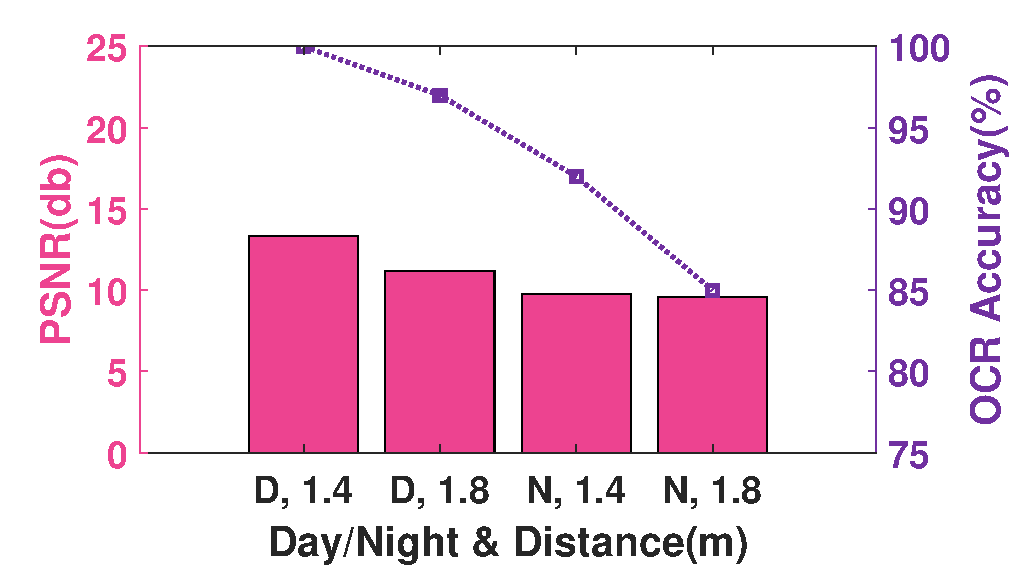
\includegraphics[width=0.40\textwidth]{./pic/data_2.pdf}\label{fig-random-1}}
%     \subfigure[Optical Lens]{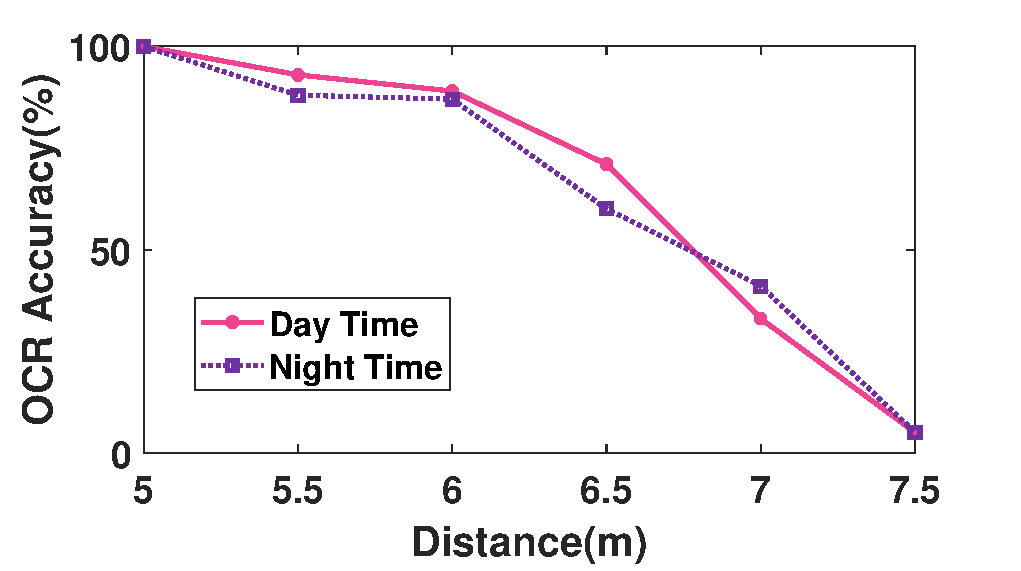
\includegraphics[width=0.40\textwidth]{./pic/data_2_2.pdf}\label{fig-random-2}}
%     \hfill
%     \caption{Performance in the random environment using traditional lens and optical Lens.}
%     \label{fig:control}
% \end{figure}

\begin{figure*}[!t]
    \centering
    \subfigure[Traditional Lens]{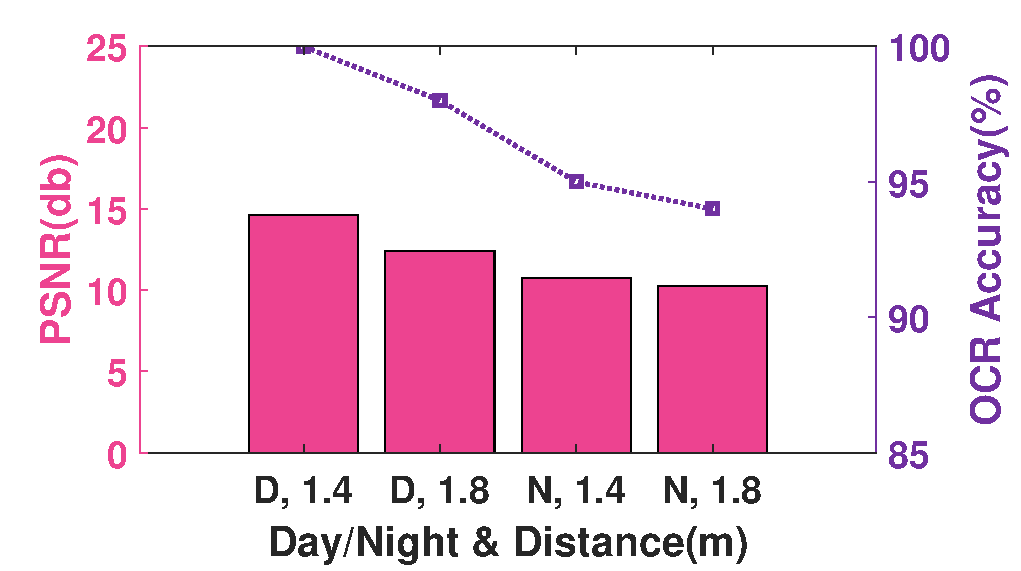
\includegraphics[width=0.24\textwidth]{./pic/data_1.pdf}\label{fig-control-1}}
    \subfigure[Optical Lens]{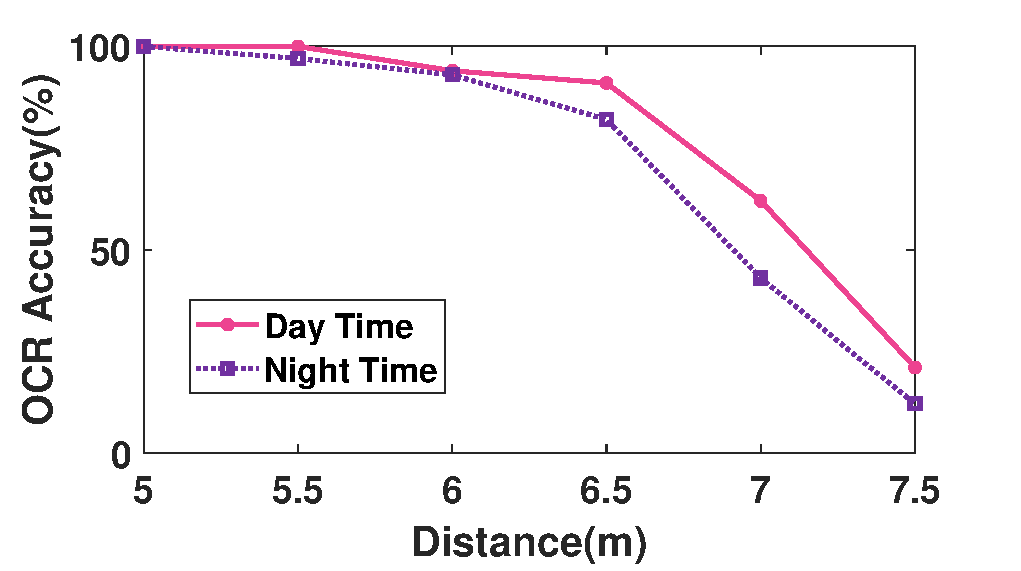
\includegraphics[width=0.24\textwidth]{./pic/data_1_2.pdf}\label{fig-control-2}}
    \subfigure[Traditional Lens]{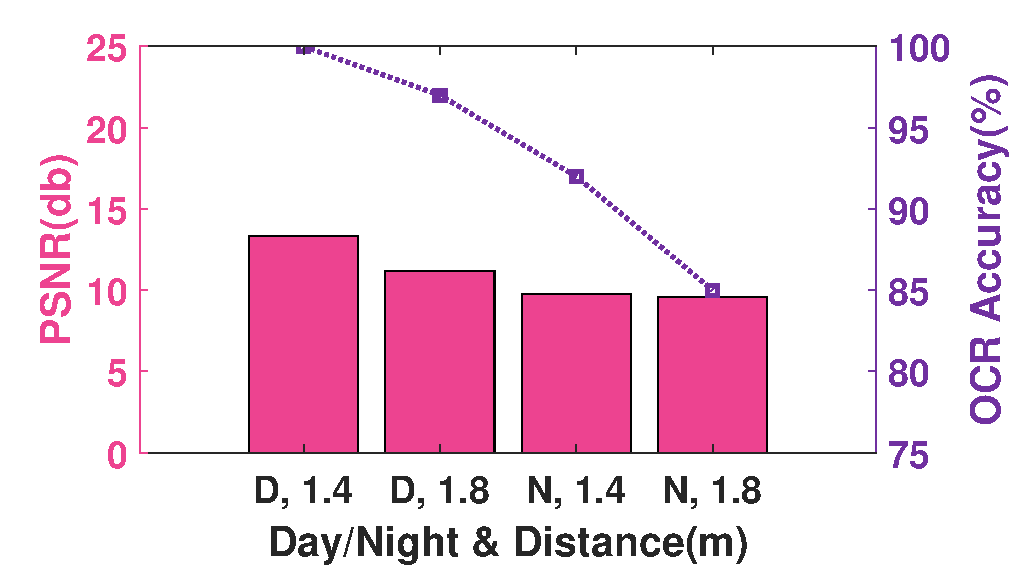
\includegraphics[width=0.24\textwidth]{./pic/data_2.pdf}\label{fig-random-1}}
    \subfigure[Optical Lens]{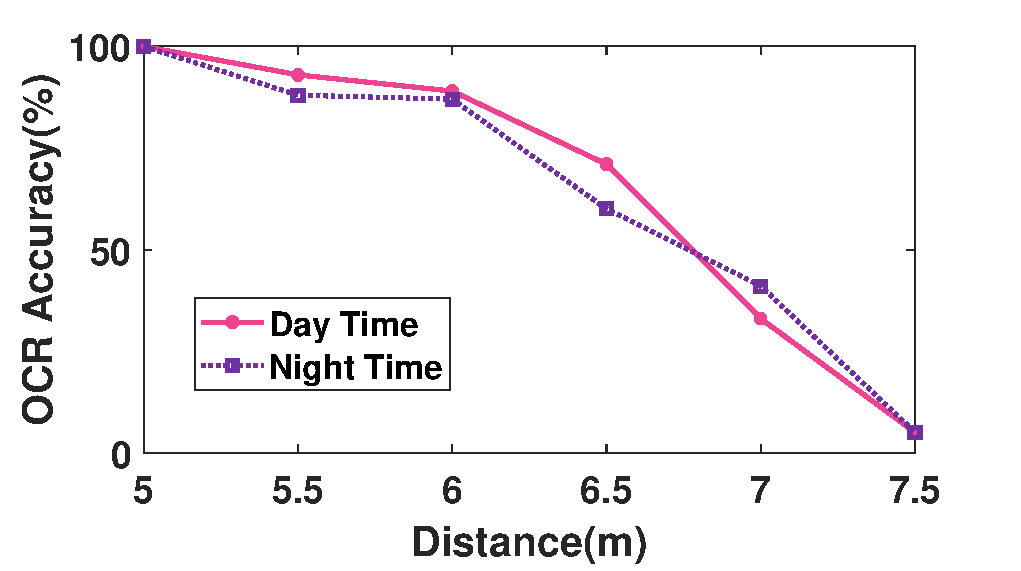
\includegraphics[width=0.24\textwidth]{./pic/data_2_2.pdf}\label{fig-random-2}}
    \hfill
    \caption{Performance in (a)(b). the random as well as (c)(d). the controlled environment using traditional lens and optical lens.}
    \label{fig:control_random}
\end{figure*}


\subsection{Performance with fewer available images}
As mentioned in sec.~\ref{sec-design}, our model is designed to work on any number of input images, the only limitation being that these images are snapshots of the same scene. This design is requisite because in certain scenarios the data displayed on the victim's screen is transient and ever-changing, e.g. password entry, where only the last character of the password is visible. We evaluated the impact of fewer available images to the performance of the SR model. The results are shown in fig.~\ref{fig:number_adapting}. We tested at the 1.8m daytime scenario for traditional lens and 6m daytime scenario for optical lens.

In the tradition lens group the performance of the model drops dramatically with fewer than 10 images, indicating that not enough input information is available to rule out all possibilities of the displayed characters. The optical lens group displayed a steady decent of accuracy when fewer images are available, which is expected, as the blur patterns are more complex and the differences between frames more pronounced, so that the images are more precious to the model and contain less overlapping data, and removing any of them will cause losses in accuracy.
\begin{figure*}[!t]
    \centering
    \subfigure[Traditional Lens]{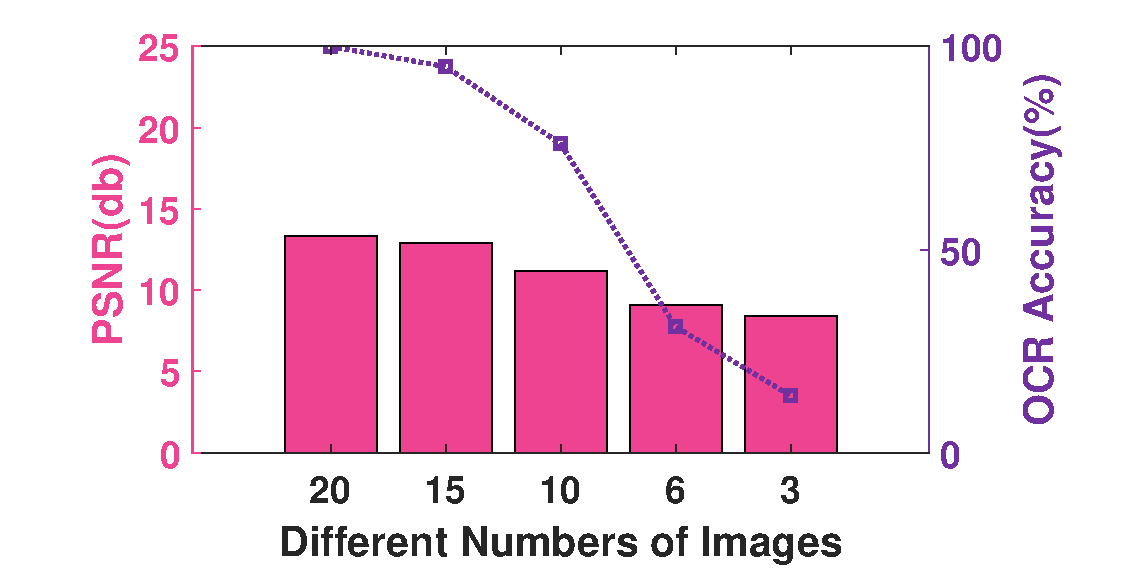
\includegraphics[width=0.24\textwidth]{./pic/data_5.pdf}\label{fig-image-tranditional-2}}
    \subfigure[Optical Lens]{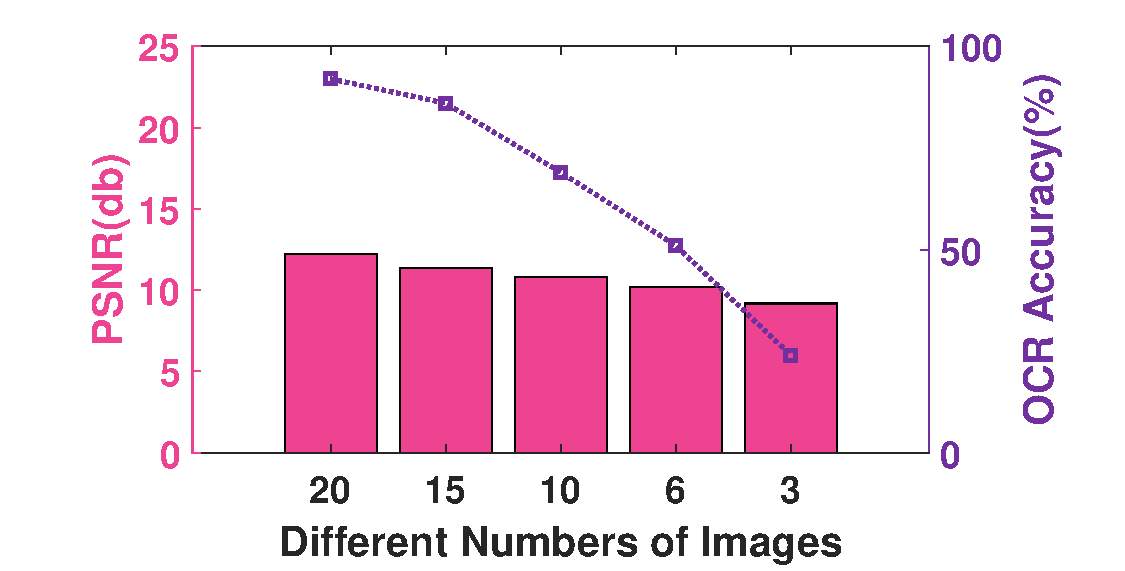
\includegraphics[width=0.24\textwidth]{./pic/data_6.pdf}\label{fig-image-optical-2}}
    \subfigure[Traditional Lens]{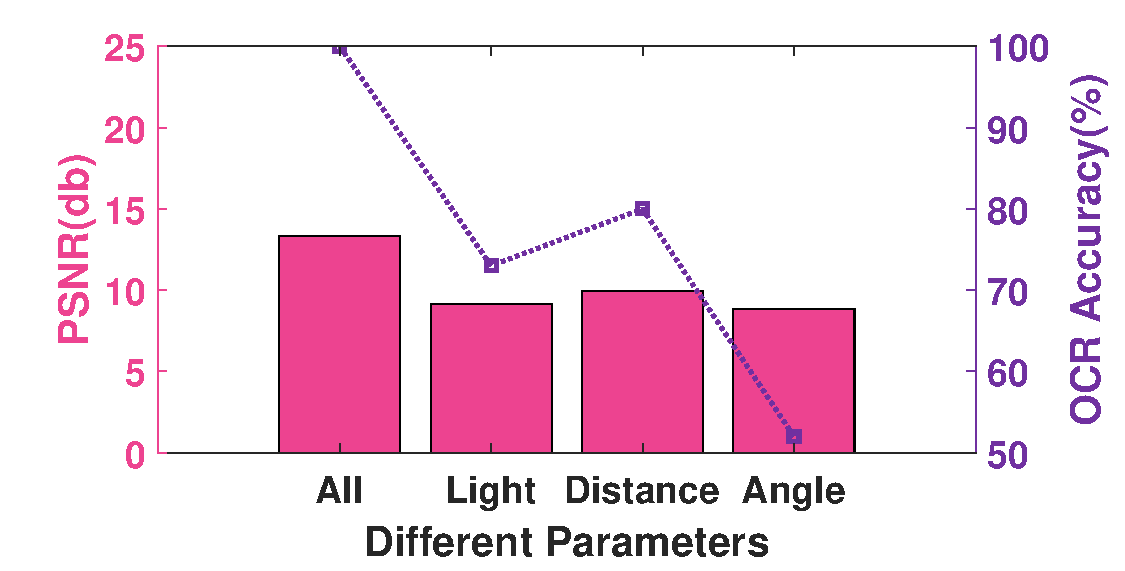
\includegraphics[width=0.24\textwidth]{./pic/data_3.pdf}\label{fig-adapt-tranditional}}
    \subfigure[Optical Lens]{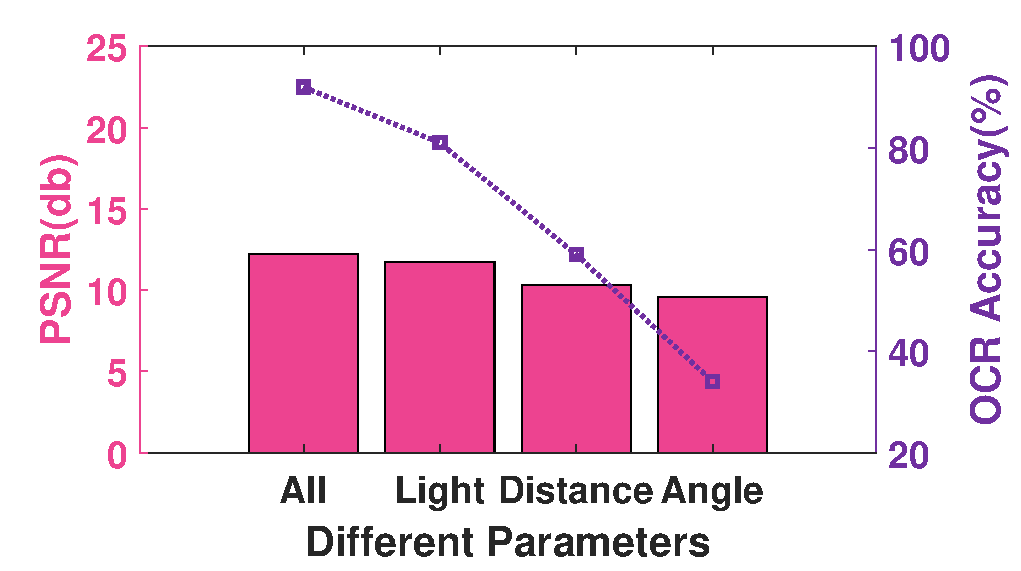
\includegraphics[width=0.24\textwidth]{./pic/data_4.pdf}\label{fig-adapt-optical}}
    \hfill
    \caption{Performance (a)(b). with fewer available images and (c)(d). for the adapting ability via traditional lens and optical lens.}
    \label{fig:number_adapting}
\end{figure*}

% \begin{figure}[!t]
%     \centering
%     \subfigure[Traditional Lens]{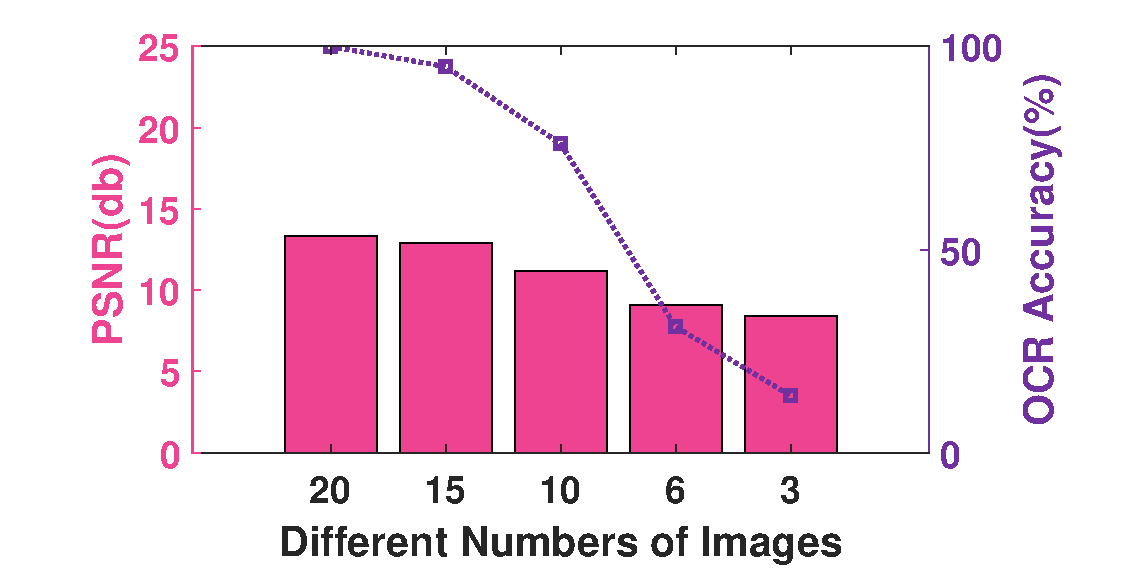
\includegraphics[width=0.40\textwidth]{./pic/data_5.pdf}\label{fig-image-tranditional-2}}
%     \subfigure[Optical Lens]{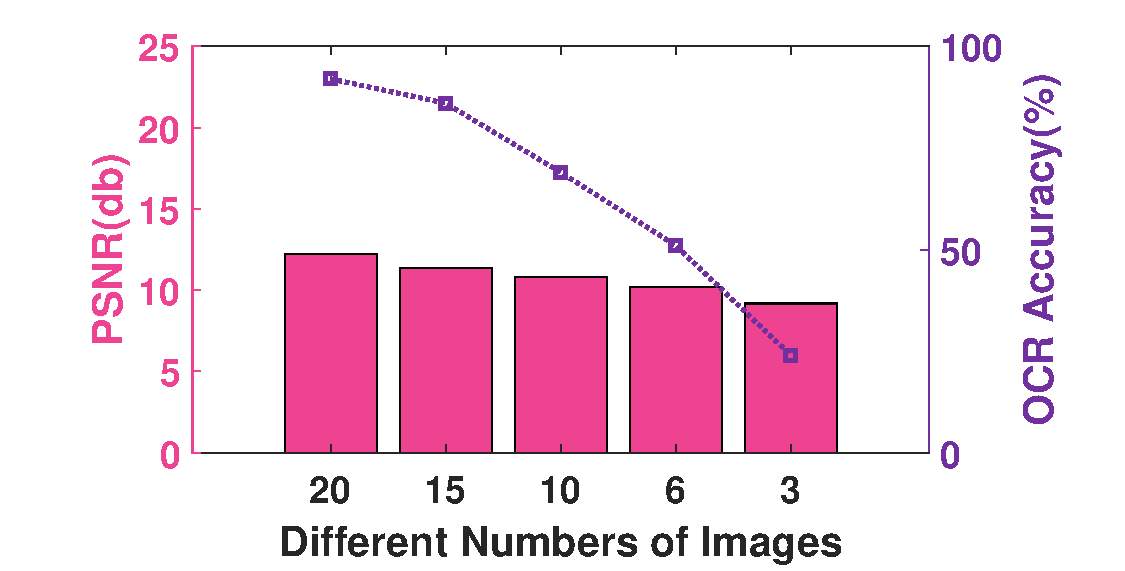
\includegraphics[width=0.40\textwidth]{./pic/data_6.pdf}\label{fig-image-optical-2}}
%     \hfill
%     \caption{Performance with fewer available images using traditional lens and optical lens.}
%     \label{fig:number}
% \end{figure}

\subsection{Adapting Ability}
We train the model with fewer groups of data, exposing it to fewer variations of environment parameters, and examine the model's performance in other environments. The results are shown in Figure~\ref{fig:number_adapting}.

We observed that variations in light and angle parameter in training data is crucial to a robust model. In the tradition lens group, the variations within 1 and 2 meters may have a smaller impact to the size of the characters
 so that features extracted at one distance might still exist at another.
 However, tilts and angles cause rotations and deformations and severely disturb the feature extraction process. The optical lens group yields similar results except at variations in distance. At a range of 6 meters, increases in distance leads to greater complexity of image blurriness, leading to more complex feature extraction and a more fragile model.
% \begin{figure}[!t]
%     \centering
%     \subfigure[Traditional Lens]{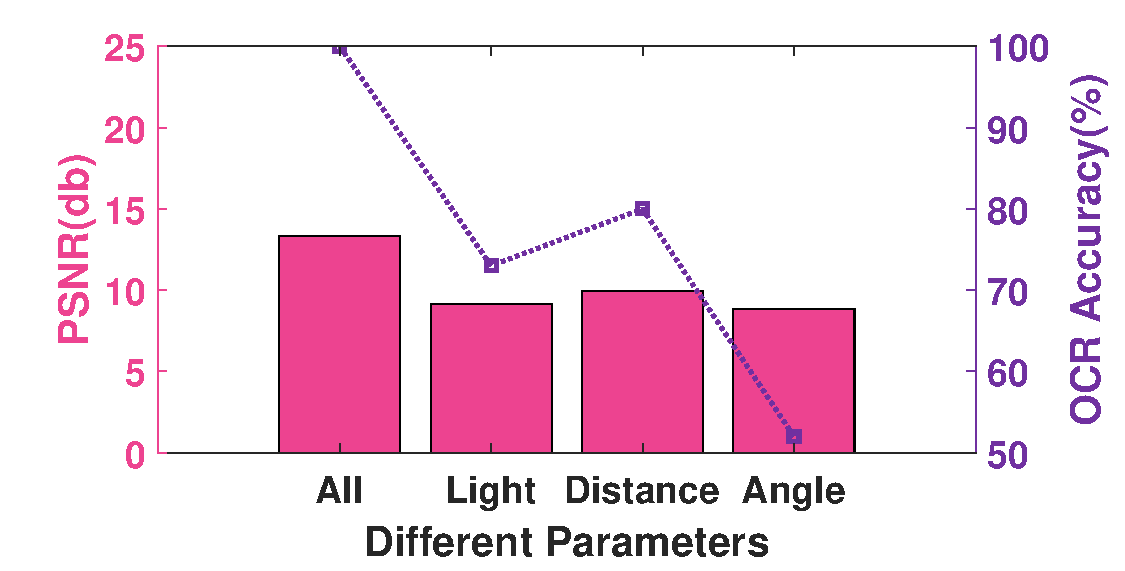
\includegraphics[width=0.40\textwidth]{./pic/data_3.pdf}\label{fig-adapt-tranditional}}
%     \subfigure[Optical Lens]{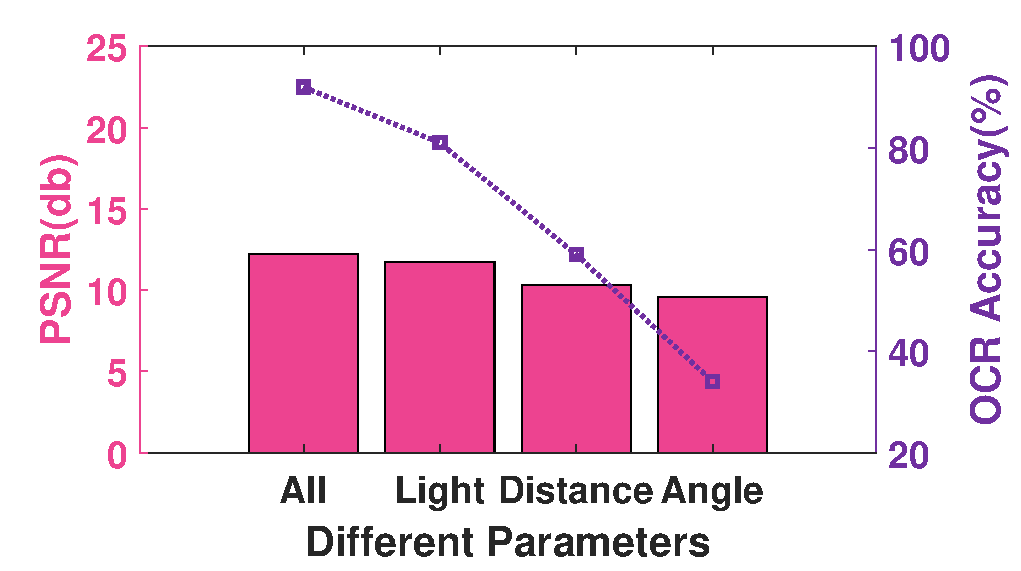
\includegraphics[width=0.40\textwidth]{./pic/data_4.pdf}\label{fig-adapt-optical}}
%     \hfill
%     \caption{Performance for the adapting ability using traditional lens and optical lens.}
%     \label{fig:adapting}
% \end{figure}

\subsection{Comparison with other architectures}
We train and test other widely used networks with the same sets of data and evaluate their results. We chose SRCNN, a commonly used single image SR network, applying it to each single image before merging the results by pixel-level average. We also used a multi-frame version of CNN consisting of 3D convolutional layers, designed for video super resolution (VideoSR). However, as mentioned above, it is very difficult for the single image approaches to utilize information and distinguish the noisy and deformed patterns, while VideoSR approaches rely upon consistency between frames, so they fail to give satisfactory results. We used the relatively easy 'daytime 1.2m-distance direct with traditional lens' group of data for testing. The results are shown in Table~\ref{table-comp}.
\begin{table}[!t]
    \centering
    \caption{Comparison with existing systems.}
    \begin{tabular}{@{}cccc@{}}
        \toprule
    System & SRPeek & SRCNN & VideoSR \\ \midrule
    PSNR & 13.32db & 7.69db & 8.403db\\ 
    OCR Accuracy & 100\% & 10\% & 23\%\\ \bottomrule
    \end{tabular}
    \label{table-comp}
\end{table}

We can see that the PSNR of SRPeek is 13.32dB which 73.2\% and 58.6\% larger than that of SRCNN and VideoSR. For the OCR accuracy, SRPeek can recognize all characters, but SRCNN and VideoSR can only recognize 10\% and 23\% of them. The results show the efficiency of our SR model in comparison with existing models.

% \section{System Evaluation}
\section{Case Study}
\label{case-study}
\subsection{Accuracy}

We build the system on smartphone and evaluate its performance in real-life scenarios (shown in Fig.~\ref{fig-reallife}). We experiment with a Redmi 6A smartphone (with a camera of 13 million pixels, no optical zooming) for the attacker and a HUAWEI Mate8 smartphone for the victim, with the former ``1.8m daytime'' setting. We ask 5 human participants to read the reconstructed characters to evaluate the usability of our model. No participants can read the unprocessed images, but all of them can decipher the information on the reconstructed image without much difficulty. The results are shown in Table~\ref{table-scenarios}.
\begin{figure}
	\centering
	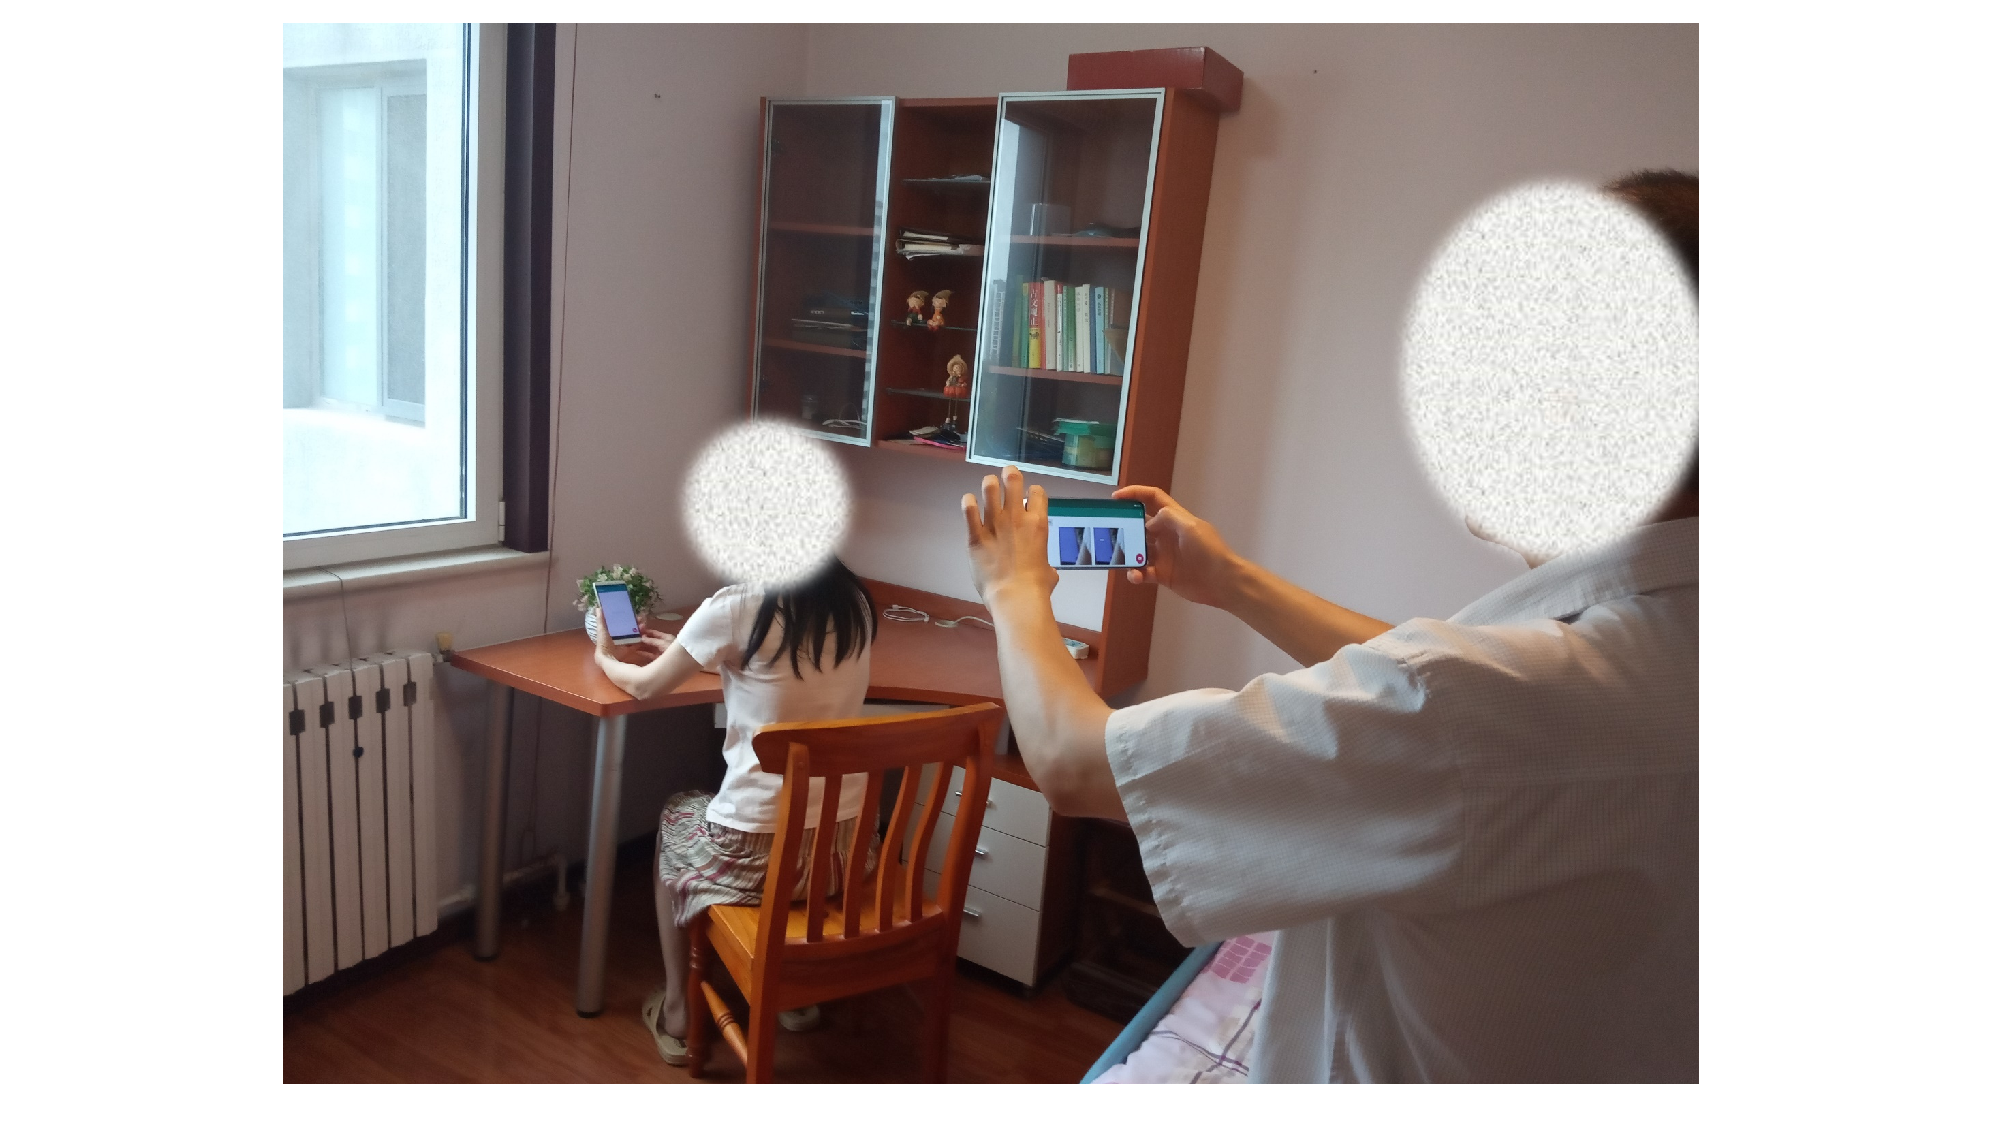
\includegraphics[width=0.80\linewidth]{pic/reallife.pdf}
    \caption{Illustration of our real-life scenario (Distance between attacker and victim is shortened for demonstration).}
	\label{fig-reallife}
\end{figure}

The results show that Human can read 95\%, 85\% and 70\% contents in home, transport and theater while the OCR accuracy is 100\%, 10\% and 23\%. That verifies human can obtain the most parts of information from the peeking in various environments. In transport, the vibration of smartphone and the darker environment can fool the OCR model for content recognition in comparison with human recognition so that leads lower accuracy in transport and theater.

\begin{table}[!t]
    \centering
    \caption{Recognition accuracy in various scenarios.}
    \begin{tabular}{@{}cccc@{}}
        \toprule
    Scenarios & Home & Transport & Theater \\ \midrule
    Naked Eye & 5\% & 0 & 0\\ 
    \midrule
    OCR & 100\% & 10\% & 23\%\\ 
    Human & 95\% & 85\% & 70\%\\ \bottomrule
    \end{tabular}
    \label{table-scenarios}
\end{table}

\subsection{Influence of hand tremors}
We ask 5 participants to capture images with handheld smartphones, keeping their hand still to their greatest effort (Handheld camera). We process these images and let them read the results. We compare this performance to the data collected on stationary phones to evaluate the influence of hand tremors.
We also ask participants to hold a smartphone in their hands and read a piece of text, without other additional instructions (Handheld target). The user may freely interact with the phone when reading. We capture images of the phone at the same time to see how our system deal with a moving target screen. The results are shown in Table~\ref{table-tremor}.

\begin{table}[!t] 
    \centering
    \caption{Impact of hand tremors when the camera (attacker phone) and/or target (victim phone) is handheld.}
    \begin{tabular}{ccccc}
        \toprule
    Accuracy & None & Camera & Target & Both  \\
    \midrule
    Naked Eye & 5\% & 0 & 5\% & 5\%\\ 
    \midrule
    OCR & 95\% & 85\% & 80\% & 80\%\\ 
    Human & 95\% & 85\% & 80\% & 85\%\\ \bottomrule
    \end{tabular}
    \label{table-tremor}
\end{table}

We can see that with the existence of tremors, the recognition accuracy drops from 95\% to 85\%/80\% for both OCR tools and human. We conclude from the results that hand tremors can impact the performance of our system. Hand tremors can cause motion blur and erratic shifts in the sub-pixel level(after image alignment phase) and impact performance.


\subsection{Success rate in different tasks}
We test the success rate of obtaining crucial information when the observed participant performs several tasks on a phone: reading text message, typing text message, entering PIN, and typing password with numbers, English and special characters(typing at 2 characters per second). We use accuracy per character as evaluation metric. In the PIN and password tasks, fewer photos will be available, but deciphering English characters is also easier than Chinese characters, and we use specifically trained models(with same structure and different training data). The results are shown in Table~\ref{table-task}.

\begin{table}[!t]
\centering
\caption{Success rate in different tasks.}
\label{table-task}
\begin{tabular}{@{}ccccc@{}}
	\toprule
Accuracy & Read text & Type text & Enter PIN & Enter password\\ \midrule
Raw Image & 5\% & 0 & 0 & 0\\
SRPeek & 100\% & 100\% & 100\% & 80\%\\ \bottomrule
\end{tabular}

\end{table}

We conclude that \textsf{SRPeek} functions normally in everyday scenarios and poses a threat to screen privacy.

\subsection{Perceived shoulder surfing susceptibility}
We ask the participants to rate the perceived shoulder-surfing susceptibility after the experiment. The attacker sits or stands at 1.8m range, pretending to be interacting with their own phone while continuously running the shoulder-surfing APP. None of the participants reported suspicion of shoulder-surfing. We believe that our system can enable a malicious attacker to gather large amounts of critical information from the victim while remaining unnoticed.




